%%
%% AUTOMATICALLY GENERATED FILE - DO NOT EDIT MANUALLY
%% File origin : Main.Rnw 
%%
\documentclass{article}

\usepackage{C:/Programs/R/current/share/texmf/Sweave}
\begin{document}
Main1
flop asd sad j
asdj 
jasd 
asd asd asd 

%% BEGIN: Content of file Sub1.Rnw

\begin{Schunk}
\begin{Sinput}
> x <- 1:10
> x
\end{Sinput}
\begin{Soutput}
 [1]  1  2  3  4  5  6  7  8  9 10
\end{Soutput}
\end{Schunk}
%% END: Content of file Sub1.Rnw



asd 
asd
asd 

asd
asd
asd

asd
asd



%% BEGIN: Content of file Sub2.Rnw

sub2
\begin{Schunk}
\begin{Sinput}
> y <- rnorm(19)
> plot(y)
\end{Sinput}
\end{Schunk}
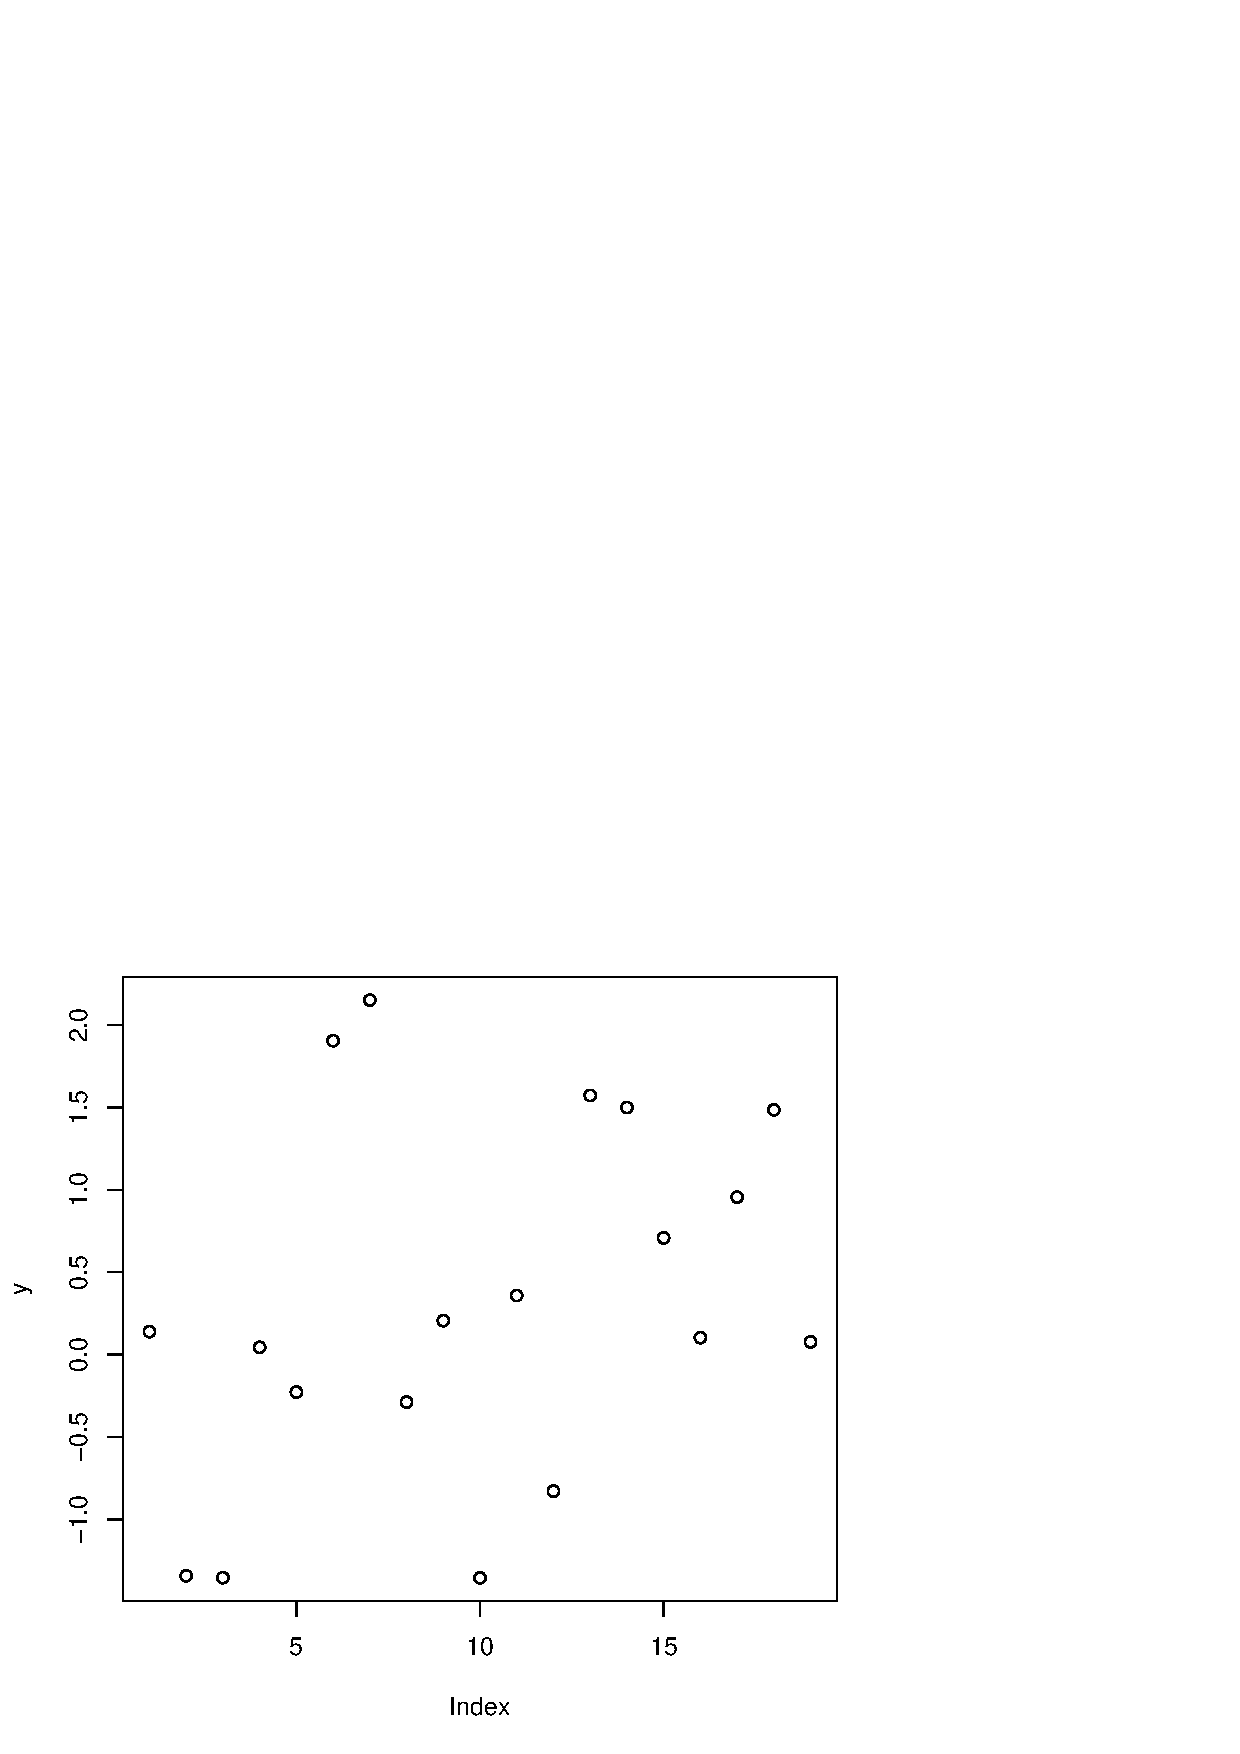
\includegraphics{fig/bar-002}

\begin{Schunk}
\begin{Sinput}
> plot(rnorm(200))
\end{Sinput}
\end{Schunk}
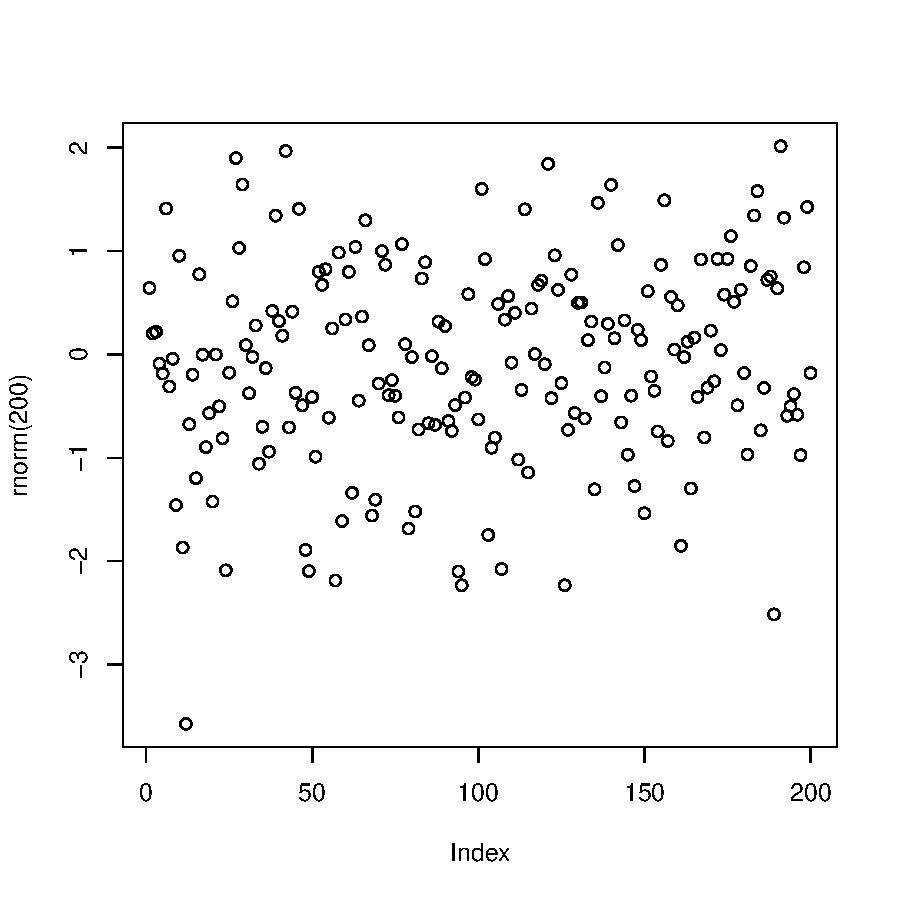
\includegraphics{fig/bar-003}

\begin{Schunk}
\begin{Sinput}
> plot(rnorm(2000))
\end{Sinput}
\end{Schunk}
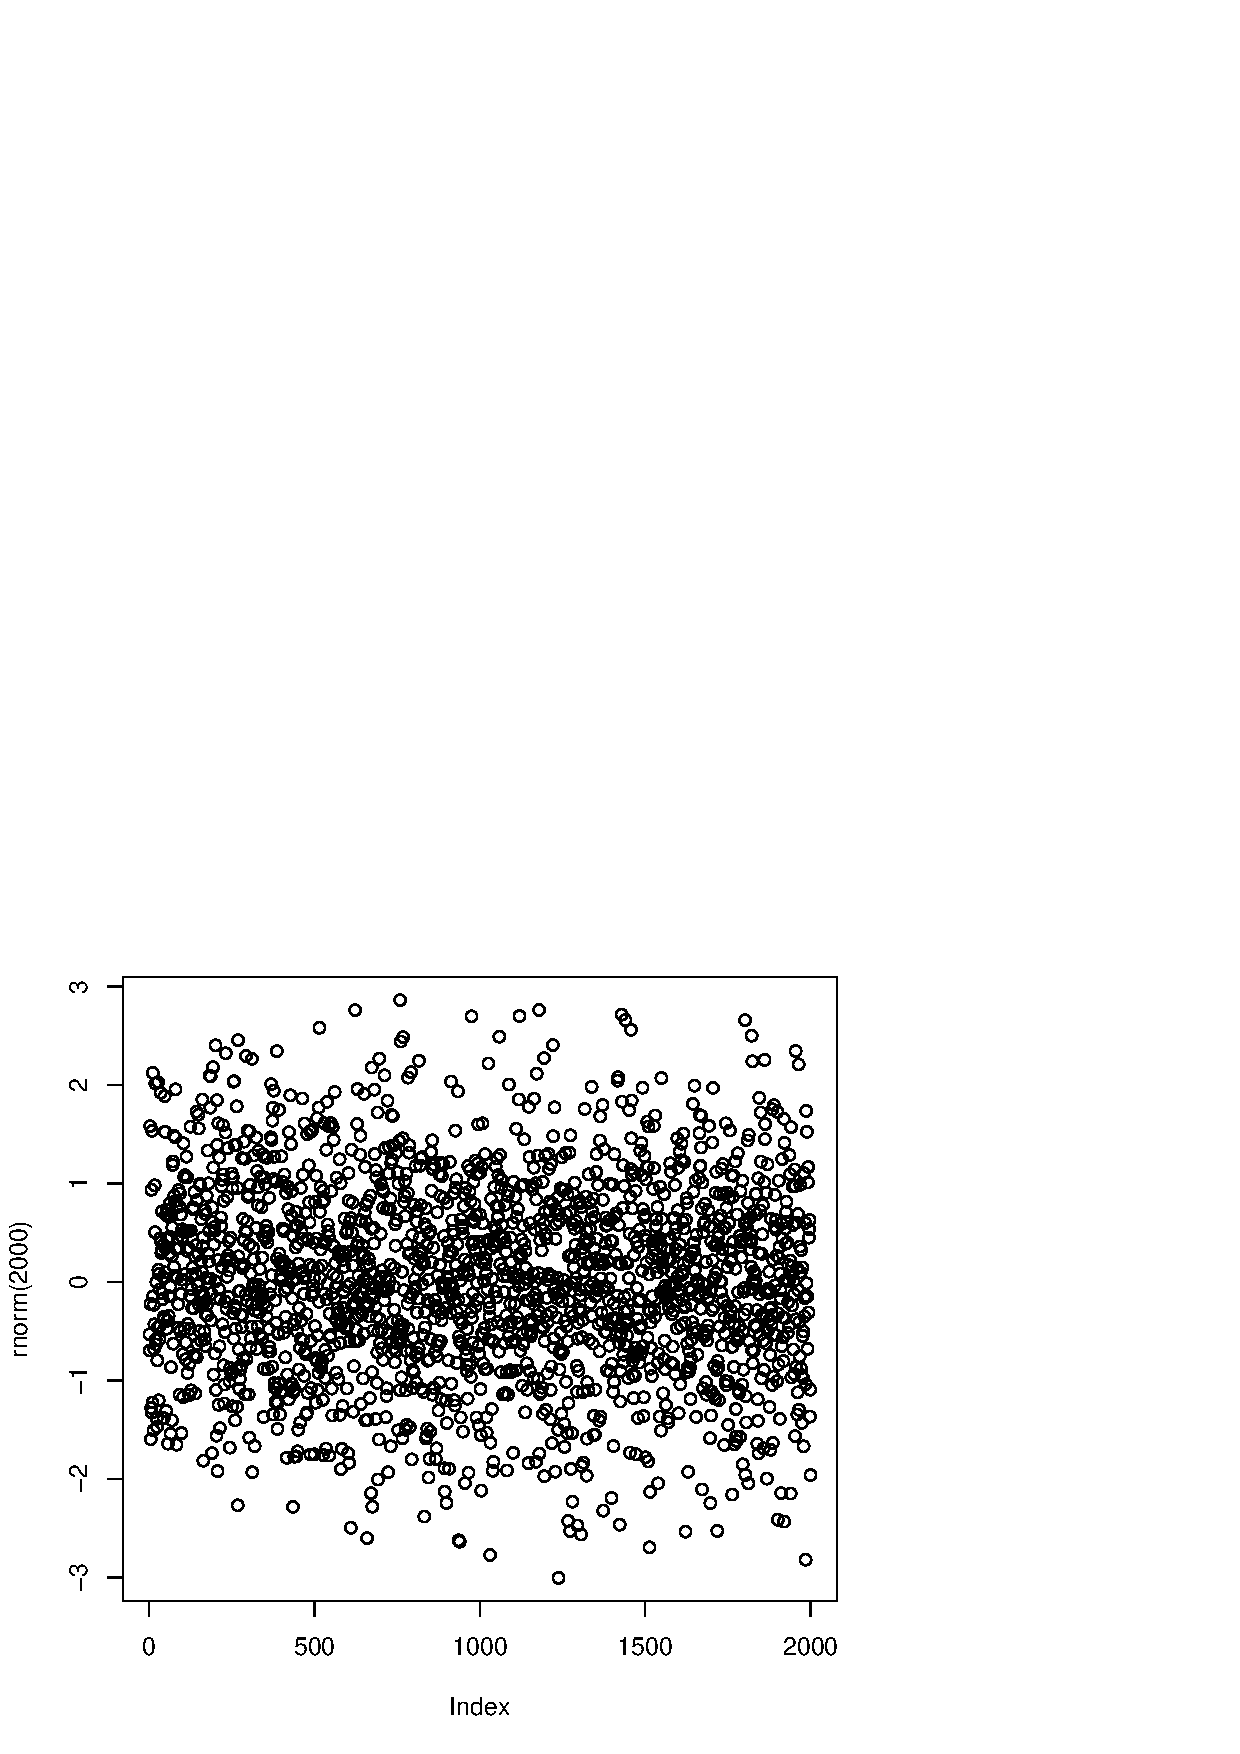
\includegraphics{fig/bar-004}

%% END: Content of file Sub2.Rnw


Main3
\end{document}

